% Define the document as a subfile and reference its root.
\documentclass[../main.tex]{subfiles}

% Begin the document.
\begin{document}
\chapter{Background} \label{ch:background}
    \section{Functional Programming and Haskell}
        Functional programming is a programming paradigm built around the evaluation of
            mathematical functions \citep{fpPaulHudak}.
        Unlike the more widely used imperative programming, which utilises a series of
            statements to alter the state of a program and produce a result, functional
            programming is based on the composition and execution of functions to produce
            that result.
        The paradigm is based on lambda calculus, a formal system of computation,
            developed by Alonzo \citet{lambdaCalculus} which is built around function
            application.
        Lambda calculus was proved to be equivalent to Turing machines by Alan
            \citet{lambdaTuringComplete}.

        One of the most widely used functional programming languages is Haskell,
            placing 31st in the TIOBE index for March 2025 \citep{tiobeIndex}.
        A statically typed, purely functional programming language, developed in the
            late 1980s, with the intention of consolidating features from existing pure
            lazy functional programming languages into a single, standardised language
            \citep{haskellHistory}.
        Haskell's namesake is Haskell Curry, who developed an equivalent system to
            lambda calculus, combinatory logic, alongside Moses Schönfinkel the 1920s and
            1930s \citep{combinatoryLogic}.
        Since its inception, there have been two major revisions of the Haskell
            language, Haskell 98 and Haskell 2010, with the latter being the most recent
            standard \citep{haskell2010}.

        Haskell is known for its use of type classes, introduced to the language by
            Phil Wadler \citep{typeClasses}.
        These allow for ad-hoc polymorphism, where functions can be defined for a set
            of types which satisfy a certain interface.
        One of the most important type classes in Haskell is the \texttt{Monad} type
            class.
        Monads provide a way to simulate effects in a pure functional language
            \citep{monads}.

    \section{Graphics}
        Computer graphics is a wide field, encompassing the use of computers for the
            creation, manipulation, and rendering of images, across both two and
            three-dimensional domains.
        Although rudimentary graphics have been around longer, making use of cathode
            ray tube displays as far back as \citet{crtBraun}, the discipline of computer
            graphics was first truly established in the 1950s and 60s \citep{graphics},
            with the development of the first viable interactive graphical displays.
        Since then, the field has grown rapidly, resulting in a plethora of techniques
            and technologies for creating and rendering graphics.

        Two-dimensional graphics are typically represented as raster graphics, where
            images are represented as a grid of pixels \citep{rasterGraphics}.
        This method of storage is simple, and reflects the same method that modern
            displays use to render images, but can result in loss of quality when images
            are scaled.
        An alternative method of storing graphics, is to use vector graphics, where
            shapes are described by mathematical equations, which are then converted into
            pixels when rendered \citep{vectorGraphics}.
        This is a more ideal solution for images which need to be scaled, as the image
            will not change in quality when resized.
        Both raster and vector graphics have their own advantages and disadvantages,
            and are used in different contexts depending on the requirements of the image.
        They are often used together, particular on websites, with raster graphics
            being used for images which require fine detail, and vector graphics being used
            for images which need to be scaled.

        \subsection{Backends for Graphics}
            \subsubsection{OpenGL}
                One of the most widely used graphics libraries is OpenGL, a cross-language,
                    cross-platform library developed by Silicon Graphics in the early 1990s
                    \citep{openGL}.
                It supports both 2D and 3D graphics, and is generally used to interact with the
                    graphics processing unit (GPU) to take advantage of hardware acceleration,
                    improving performance particularly for 3D graphics, but can also be used for
                    central processing unit (CPU) rendering.
                With several hundred procedures available within the API, OpenGL is a both a
                    powerful and versatile library, making it ideal for a wide range of
                    applications, from video games to scientific visualisation.

            \subsubsection{Cairo}
                Cairo is a 2D graphics library, designed to be both fast and portable
                    \citep{cairo}.
                It is designed to produce consistent results across different platforms, and
                    supports a wide range of output formats, including raster graphics, vector
                    graphics, and PDFs.
                Although implemented in C, Cairo has bindings available for a number of
                    languages, including Haskell, making it a versatile library for generating
                    graphics.

        \subsection{Graphics in Haskell}
            \subsubsection{Gloss}
                There are a number of libraries and bindings available for Haskell which aid in
                    generating graphics.
                One of the most popular of these, with a rating on Hackage of 2.75 out of 3 and
                    69,490 downloads, is the Gloss library, which provides a simple interface for
                    creating graphics in Haskell \citep{hackageGloss}.
                As with many graphics libraries, Gloss uses OpenGL as its rendering engine, but
                    provides a simpler and higher-level interface, making it ideal for beginners or
                    for quick sketches.
                Due to the simplicity of Gloss, there are a limited number of functions
                    available, which can make it difficult to create more complex graphics.

            \subsubsection{Diagrams}
                Another popular Haskell graphics library is Diagrams \citep{hackageDiagrams},
                    which also has a Hackage rating of 2.75, but has fewer downloads than Gloss, at
                    34,898 \citep{hackageDiagrams}.
                This provides a more powerful and flexible interface than Gloss, by allowing
                    the user to choose from one of six backends, including Cairo, but not OpenGL.
                Diagrams' larger API makes it less beginner-friendly but more versatile due to
                    its multiple backends.

        \subsection{Graphics in Web Browsers}
            The first web browser, originally named WorldWideWeb before becoming Nexus, was
                developed by Sir Tim \citet{worldWideWeb}, alongside the first web server, and
                a basic version of HyperText Markup Language (HTML) \citep{html}.
            Web browsers are inherently designed for rendering structured graphical
                content, and while the first browsers were limited to displaying just HTML,
                developments in the last three decades, including the introduction of Cascading
                Style Sheets (CSS) \citep{css}, JavaScript \citep{js}, and HTML5 \citep{html5},
                have allowed for far more complex and interactive graphics.

            \subsubsection{Scalable Vector Graphics (SVGs)}
                Scalable Vector Graphics (SVGs) use an XML-based format, similar to HTML, to
                    describe two-dimensional vector graphics \citep{svg}.
                Each object in an SVG is appended to the Document Object Model (DOM) of the web
                    page, allowing the browser to automatically re-render the image if any changes
                    are made to the SVG.

            \subsubsection{HTML5 Canvas API}
                The \texttt{canvas} element was first introduced by Apple in 2004
                    \citep{appleCanvas}, before being later standardised in the HTML5 specification
                    \citep{html5Canvas} in 2011.
                By itself, the \texttt{canvas} element is nothing but a plain bitmap image.
                Where it becomes interesting, however, is when it is combined with JavaScript,
                    allowing for the dynamic generation and rendering of graphics.
                Unlike SVGs, each component that makes up the image is not stored in the DOM,
                    but is rendered directly to the canvas, which can result in better performance
                    once the image is rendered, but requires the whole canvas to be redrawn if any
                    changes are made.

            \subsubsection{WebGL}
                WebGL brings the capabilities of OpenGL to web browsers, allowing for
                    hardware-accelerated 2D and 3D graphics to be rendered without the need for any
                    plugins \citep{webGL}.
                Before being standardised by the Khronos Group, WebGL started out as two
                    independent experiments by Mozilla and Opera \citep{mozillaWebGL, operaWebGL}.
                WebGL renders inside the \texttt{canvas} element, and is based on OpenGL ES
                    2.0, a subset of OpenGL which is designed for embedded systems
                    \citep{openGLES}.

    \section{Existing Work}
        This section will discuss two existing tools which provide web-based
            environments for creating graphics.
        The first, P5.js, is a JavaScript library which provides a simple interface for
            creating graphics in web browsers, and has its own web-based editor.
        The second, CodeWorld, is a tool which provides both a block-based and a
            Haskell-like interface for creating graphics in Haskell.
        These served as bases for the development of the tool described in this report.

        \subsection{Processing and P5.js}
            \begin{figure}[H]
                \centering
                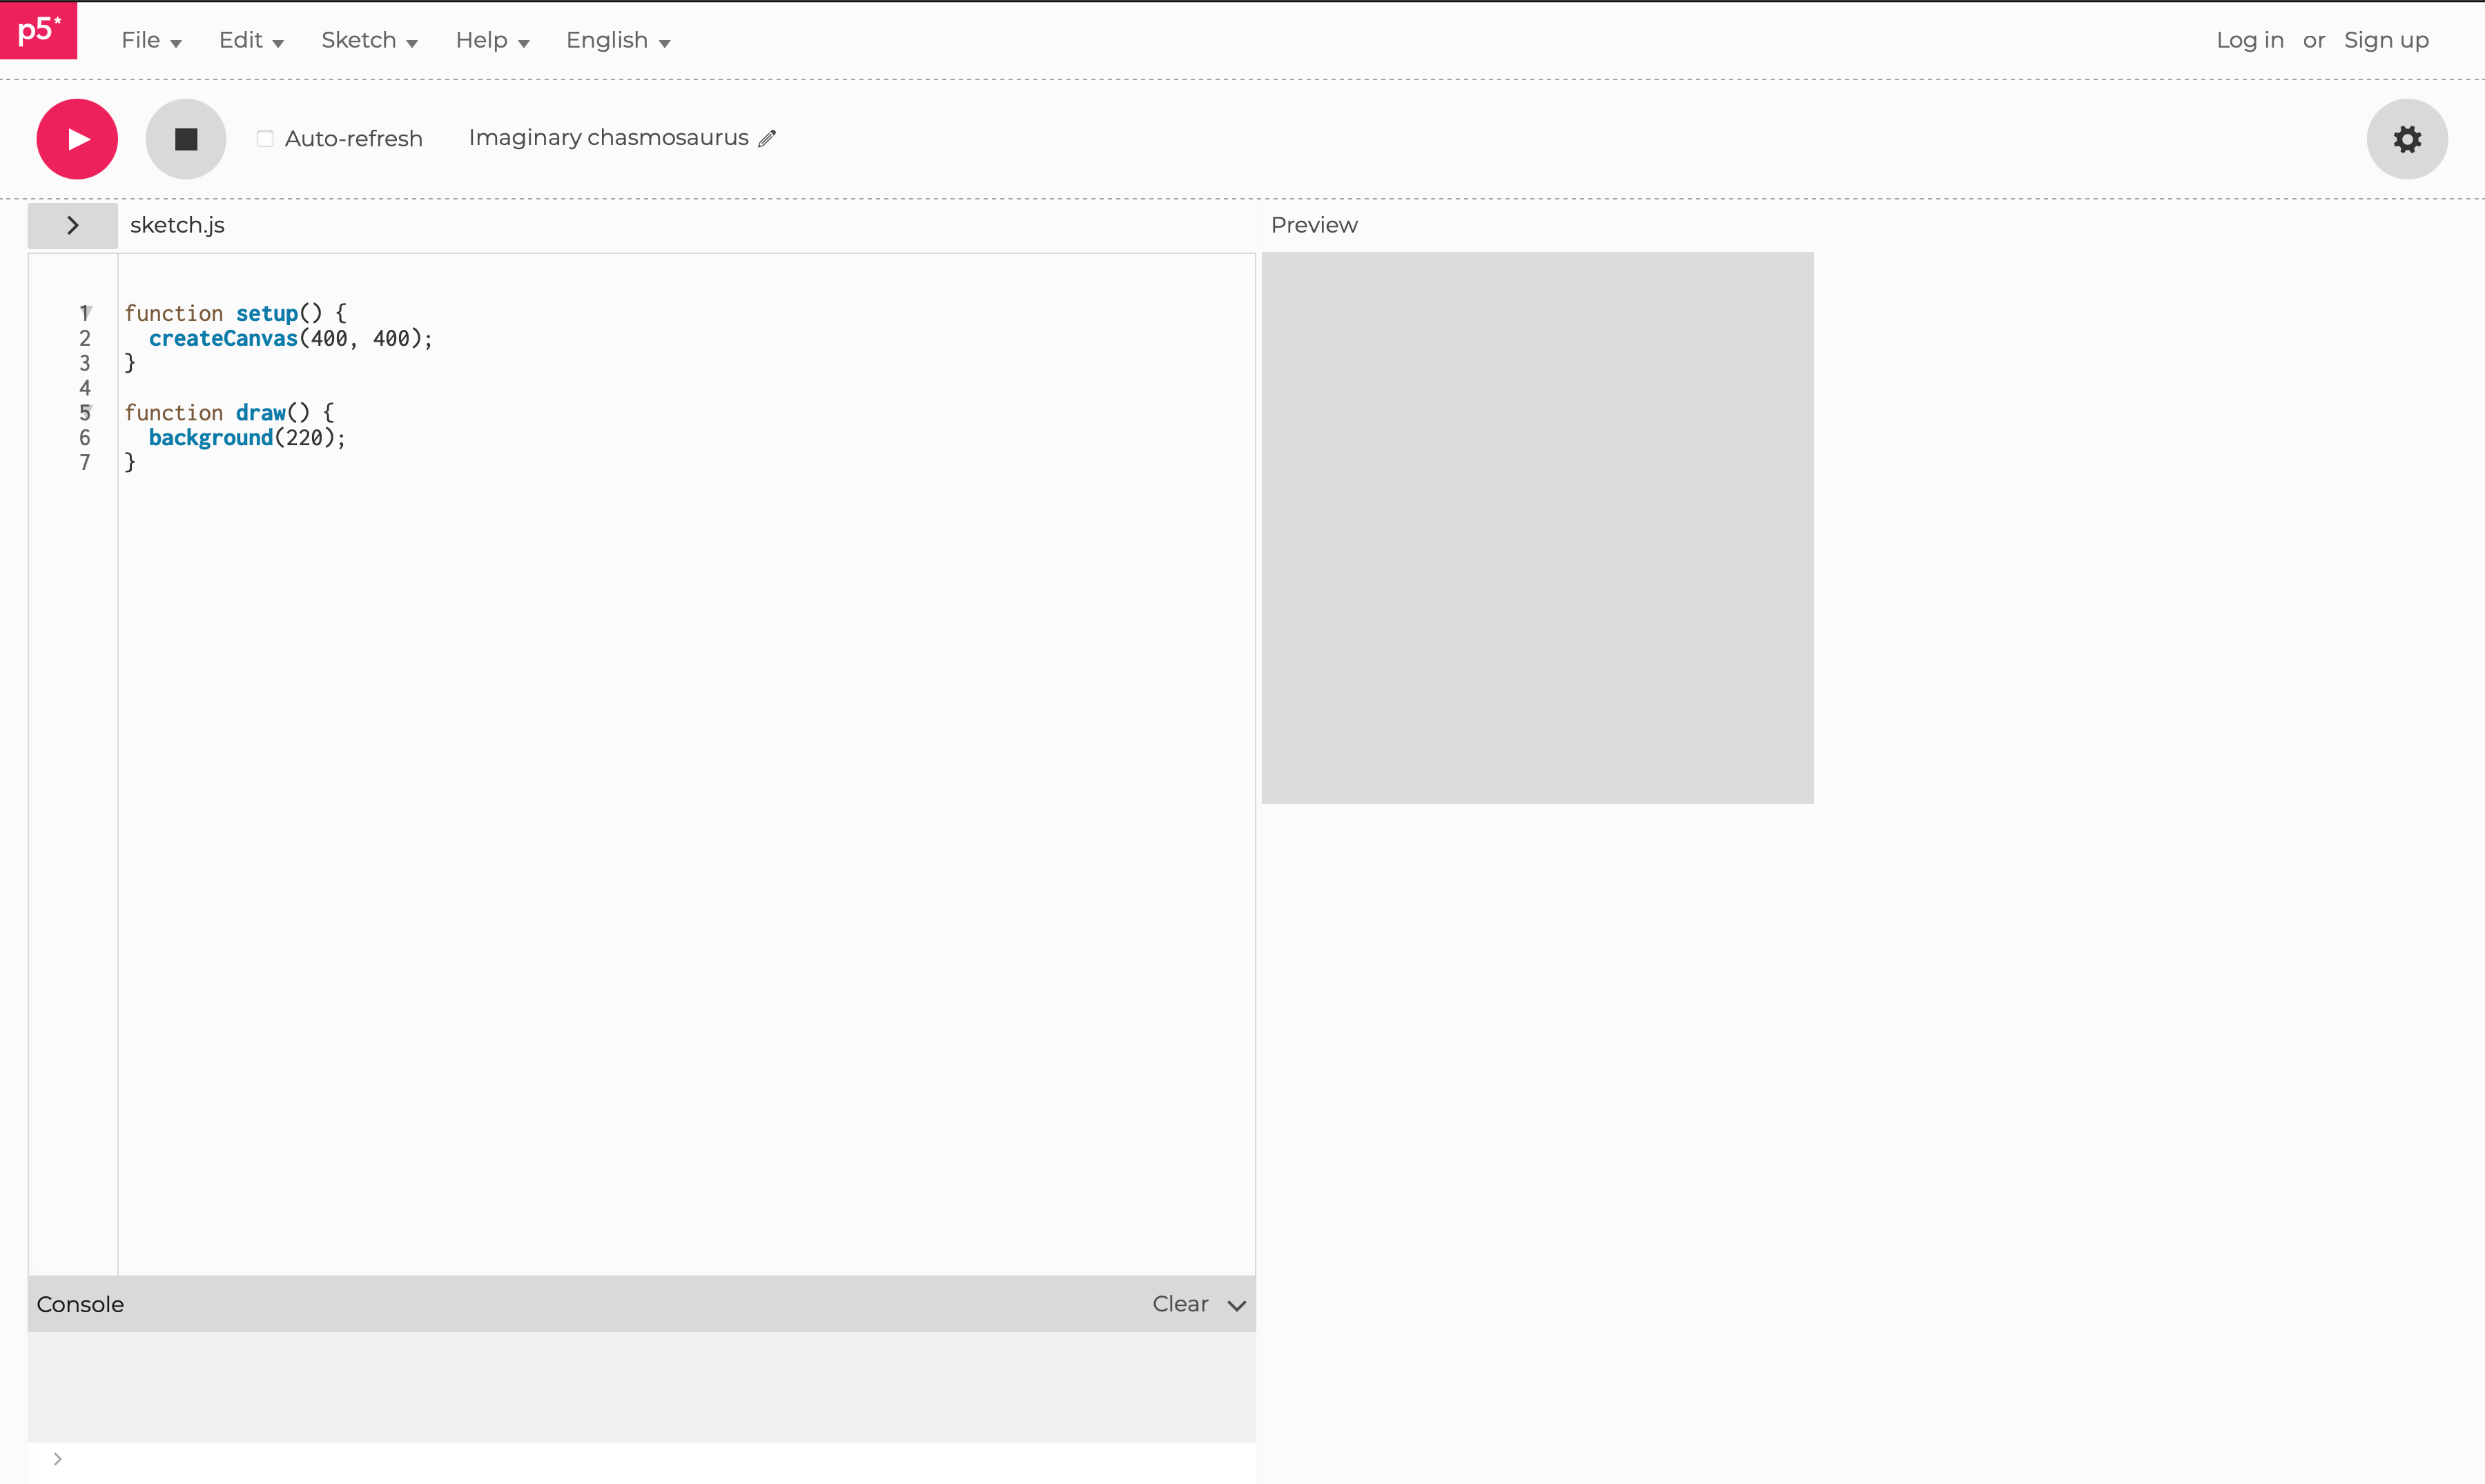
\includegraphics[width=0.75\textwidth]{p5.png}
                    \caption{The P5.js editor.}
                    \label{fig:p5}
            \end{figure}

            Processing is a programming language and integrated development environment
                (IDE) based on Java (with bindings available for JavaScript, Python and Ruby),
                allowing for the creation of graphics and animations \citep{processing}.
            P5.js is the official JavaScript binding for Processing, which uses the web
                browser to display graphics via the HTML \texttt{canvas} element \citep{p5js}.
            Processing and P5.js sketches are built around two core functions:
                \texttt{setup()} which runs once at the start, and \texttt{draw()} which
                executes repeatedly to update the canvas.
            While Processing uses OpenGL as its rendering engine, P5.js uses the HTML5
                Canvas API, with WebGL support available as an opt-in feature \citep{p5WebGL}
                to improve performance and enable 3D graphics.

            While there is no official support for Haskell from the Processing Foundation,
                there have been some unofficial bindings published on Hackage.
            One such package is processing by \citet{hackageProcessing}, which uses p5.js
                as a backend, producing its output using the HTML5 \texttt{canvas} element, but
                this was last updated in 2016, and has seemingly been abandoned.
            Another package, processing-for-haskell by \citet{hackageProcessingForHaskell},
                was last updated in 2022, and implements almost the entire Processing API in
                Haskell, using OpenGL as the backend, just as the original Processing does, but
                does not support generating graphics in web browsers.

        \subsection{CodeWorld}
            \begin{figure}[H]
                \centering
                \includegraphics[width=0.75\textwidth]{codeworld.png}
                    \caption{The CodeWorld editor.}
                    \label{fig:codeworld}
            \end{figure}

            CodeWorld is an educational website distributed by Google and created by Chris
                \citet{codeWorldGitHub}, which provides an environment for creating simple
                graphics using Haskell.
            It uses GHCJS, a Haskell to JavaScript compiler, to compile Haskell code into
                JavaScript, which is then executed in the browser.

            There are three variants of CodeWorld available:
            \begin{itemize}
                \item The first (\texttt{https://code.world}) uses an educational, simplified
                      version of Haskell 98, with some features removed to make it easier for
                      beginners to learn.
                \item The second (\texttt{https://code.world/haskell}) uses a full version of
                      Haskell 2010.
                \item The third (\texttt{https://code.world/blocks}) uses a drag and drop block
                      editor, designed for beginners who are not yet comfortable writing code.
                      This version is not yet stable, and is not recommended for use.
            \end{itemize}

\end{document}
